\documentclass[a4paper,titlepage,12pt]{scrartcl}	%El modo de documento es para la numeración.

\usepackage{graphicx} %Imágenes
\usepackage[utf8]{inputenc} %Tildes
\usepackage[spanish,es-tabla]{babel} %Español, es-table: llamar tablas en vez de cuadros
\usepackage[breaklinks=true]{hyperref} %Hiperenlaces
\usepackage{amssymb, amsmath, amsbsy} %Símbolos matemáticos
\usepackage{float} %Mover las imágenes usando [H]
\usepackage{eurosym} %Símbolo de euro \euro
\usepackage{listings} %Código

\numberwithin{figure}{section} %Hace que la primera figura de cada sección X sea X.1
\numberwithin{table}{section} %Hace que la primera tabla de cada sección X sea X.1

\begin{document}
	\begin{titlepage}
		\begin{center}
			\begin{figure}[htb]
				\begin{center}
					
\includegraphics[width=12cm]{./Portada/ugr.png}
				\end{center}
			\end{figure}

			\vspace*{0.8cm}
			\begin{Large}
				\textbf{Grado en Ingeniería Informática.}\\
			\end{Large}
			\begin{Huge}
				\vspace{1.5cm}
				\textbf{Práctica 1.} \\
			\end{Huge}
			\vspace*{0.76cm}
			\rule{100mm}{0.1mm}\\
			\vspace*{0.5cm}
			\begin{large}
				\textbf{Nombre de la asignatura:}\\
				Ingeniería de Servidores.\\
				\vspace*{0.5cm}
				\textbf{Realizado por:}\\
				Néstor Rodríguez Vico \\

				\vspace*{2cm}
				\begin{figure}[htb]
					\begin{center}
						
\includegraphics[width=5cm]{./Portada/etsiit.png}
					\end{center}
				\end{figure}
				\vspace*{-0.6cm}
				ESCUELA TÉCNICA SUPERIOR DE INGENIERÍAS INFORMÁTICA Y DE TELECOMUNICACIÓN.\\
				\rule{20mm}{0.1mm}\\
				\vspace*{0.6cm}
				Granada, \today.
			\end{large}
		\end{center}
	\end{titlepage}
	
	%--------------Indices--------------
	\tableofcontents
	\clearpage
	\listoffigures %Imagenes
	\clearpage
	\listoftables %Tablas
	\clearpage
	%----------------------------------
	
	\section[¿Qué modos y/o tipos de “virtualización” existen? (no más de tres párrafos)]{¿Qué modos y/o tipos de “virtualización” existen? (no más de tres párrafos)}
	
	Como dicen Oracle y RedHat, existen tres tipos de virtualización: \cite{VirtualizacionOracle} \cite{VirtualizacionRH}
	
	\begin{itemize}
		\item \textbf{Virtualización total: }
		La máquina virtual simula el hardware donde se ejecuta. De este modo, el sistema puede ejecutarse correctamente sin tener que modificar el sistema operativo anfitrión.		
		
		\item \textbf{Para-virtualización: } Implica ejecutar versiones modificadas del sistema operativo. El sistema para-virtualizado es modificado para saber de que está siendo virtualizado, ofreciendo así un incremento de posibilidades en cuanto a optimización ya que el la máquina virtual es más consciente de su entorno. El rendimiento es muy cercano al que se obtendría ejecutando el sistema operativo sin virtualizar.
		
		\item \textbf{Driver para-virtualizados: } Los dos tipos anteriores pueden ser combinados para permitir que sistemas operativos sin modificar alcancen un rendimiento de operaciones de entrada y salida alto usando drivers para-virtualizados en sistemas operativos completamente virtualizados. \\
		En el caso de RedHat \cite{VirtualizacionRH} estos drivers contienen los drivers de almacenamiento y de red para máquinas virtuales de Microsoft Windows® completamente virtualizados. Estos driver permiten que la máquina de Microsoft Windows® se ejecute Red Hat Enterprise Linux con un rendimiento en operaciones de disco y de red mejorados.
	\end{itemize}
	
	\section[Muestre los precios y características de varios proveedores de VPS (Virtual Private Server) y compare con el precio de servidores dedicados (administrados y no administrados). Comente diferencias.]{Muestre los precios y características de varios proveedores de VPS (Virtual Private Server) y compare con el precio de servidores dedicados (administrados y no administrados). Comente diferencias.}
	
	Para poder comparar los proveedores más fácilmente, vamos a coger la opción más cara y con más prestaciones de cada proveedor. Primero vamos a comprar los proveedores de VPS:
		
	\begin{table}[H]
		\centering
		\begin{tabular}{|c|c|c|c|}
			\hline
			& Hostalia \cite{HostaliaVPS} & RoseHosting \cite{RoseHostingVPS} & Bluehost \cite{BluehostVPS}\\
			\hline
			Nº de procesadores & 2 procesadores XEON & 10 CPU Cores & 4 CPU Cores\\
			\hline
			Disco & 100GB & 500GB SSD & 240GB SAN\\
			\hline
			RAM & 3GB & 32GB & 8GB\\
			\hline
			Tráfico & 1000GB & No medido & 4TB\\
			\hline
			Precio & 26.21 \euro & 354.95 \euro & 59.99 \euro\\
			\hline
		\end{tabular}
		\caption[Proveedores VPS.]{Proveedores VPS.}
	\end{table}
	
	A continuación vamos a comprar servidores dedicados no administrados:
	
	\begin{table}[H]
		\centering
		\begin{tabular}{|c|c|c|c|}
			\hline
			& DinaHosting \cite{DinahostingNoAdministrado} & Rubinhost \cite{RubinhostNoAdministrado} & Nominalia \cite{NominaliaNoAdministrado}\\
			\hline
			Modelo del procesador & 2xE5-2640v3 & 1xE5-1410v2 & 2xE5-2640-v4\\
			\hline
			Disco & 1.2TB & 2x4TB/2x500GB SSD & 4x1TB 2.5SATA\\
			\hline
			RAM & 32GB & 96GB & 64GB\\
			\hline
			Tráfico & Ilimitado & Ilimitado & 30TB\\
			\hline
			Precio & 360.82 \euro & 129.99 \euro & 215 \euro\\
			\hline
		\end{tabular}
		\caption[Proveedores de servidores dedicados no administrados.]{Proveedores de servidores dedicados no administrados.}
	\end{table}
	
	Y finalmente vamos a comparar los servidores dedicados administrado:
	
	\begin{table}[H]
		\centering
		\begin{tabular}{|c|c|c|c|}
			\hline
			& DinaHosting \cite{DinahostingAdministrado} & Rubinhost \cite{RubinhostAdministrado} & Axarnet \cite{AxarnetAdminitrado}\\
			\hline
			Modelo del procesador & 2xE5-2640v3 & 1xE5-1410v2 & 2xE5-2420\\
			\hline
			Disco & 1.2TB & 2x4TB/2x500GB SSD & 4x600GB SAS\\
			\hline
			RAM & 32GB & 96GB & 32GB\\
			\hline
			Tráfico & Ilimitado & Ilimitado & Ilimitado\\
			\hline
			Precio & 423.38 \euro & 129.99 \euro & 299 \euro\\
			\hline
		\end{tabular}
		\caption[Proveedores de servidores dedicados administrados.]{Proveedores de servidores dedicados administrados.}
	\end{table}
	
	La mayor diferencia que nos encontramos es en dos temas, coste y prestaciones. El coste de los servidores dedicados es bastante más alto, a excepción de RoseHosting \cite{RoseHostingVPS}. Podemos ver que el proveedor VPS más barato cuesta 26.21 \euro/mes mientras que el servidor dedicado más barato cuesta 129.99 \euro/mes. En cuanto a prestaciones sucede igual, la mejor opción de un proveedor VPS tiene 32GB de RAM y 500GB SSD de disco mientras que la mejor opción de un servidor dedicado tiene 96GB de RAM y 2x500GB SSD de disco.
	
	\section[Cuestión 3.]{Cuestión 3.}
	
	\subsection[a) Enumere y explique brevemente al menos tres de las innovaciones en Windows Server 2016 y 2012 R2 respecto a 2008R2.]{\textbf{a)} Enumere y explique brevemente al menos tres de las innovaciones en Windows Server 2016 y 2012 R2 respecto a 2008R2.}
	En la página de Microsoft \cite{DiferenciasWindowsServer} podemos ver todas las diferencias entre las tres versiones de Windows Server previamente mencionadas. Tres de ellas son:
	\begin{itemize}
		\item \textbf{Windows Defender: } Se trata del antivirus desarrollado por Windows. Tanto en Windows Server 2008 R2 y Windows Server 2012 R2 estaba parcialmente soportado mientras que en Windows Server 2016 está soportado completamente.
		\item \textbf{AppLocker: } Dicha característica permite bloquear aplicaciones para que solicite una contraseña al intentar abrir la aplicación. En Windows Server 2008 R2 estaba parcialmente soportado mientras que en Windows Server 2012 R2 y 2016 está soportado completamente.
		\item \textbf{Software Load Balancer: } Dicha característica permite balancear la carga del servidor. En Windows Server 2008 R2 no estaba soportado, en Windows Server 2012 R2 se soportó parcialmente mientras que en Windows Server 2016 está soportado completamente.
	\end{itemize}

	\subsection[b) ¿Qué es Windows Server 2016 nano?]{\textbf{b)} ¿Qué es Windows Server 2016 nano?}
	Nano Server es un servidor administrado de forma remota que ejecuta un sistema operativo optimizado para servicios privados en la nube y \textit{datacenters}. Es similar a Windows Server en el modo Server Core, pero significantemente más pequeño y sólo soporta aplicaciones de 64-bits. Ocupa menos espacio en disco, se configura mñas rapido y requiere menos actualizaciones y reinicios que Windows Server. Cuando es necesario un reinicio, se reinicia más rápido. La instalación de Windows Server Nano esta disponible para las ediciones \textit{Standard} y \textit{Datacenter} de Windows Server 2016. \cite{WindowsServerNano}
	

	\section[¿Qué son los productos MAAS y Landscape ofrecidos por Canonical (la empresa que desarrolla Ubuntu)?]{¿Qué son los productos MAAS y Landscape ofrecidos por Canonical (la empresa que desarrolla Ubuntu)?}
	
	\begin{itemize}
		\item \textbf{MAAS (Metal as a Service):} permite configurar un servidor desde cero, esto es, partir de sólo el hardware, sin ni si quiera un sistema operativo instalada hasta conseguir un servidor completamente funcional y listo para que el usuario pueda ejecutar sus programas en el. \cite{MASSUbuntu} \cite{MASS}
		
		\item \textbf{Landscape:} es la principal herramienta de gestión para implementar, supervisar y gestionar un servidor de Ubuntu. \cite{Landscape}
	\end{itemize}
	
	\section[¿Qué relación tiene esta distribución con Red Hat y con el proyecto Fedora?]{¿Qué relación tiene esta distribución con Red Hat y con el proyecto Fedora?}
	
	La distribución CentOS Linux es una plataforma estable derivada de las fuentes de Red Hat Enterprise Linux (RHEL). \cite{CentOS} La relación surge cuando, el 7 de Enero de 2014, CentOS realizó una publicación indicando que unía sus fuerzas al equipo de Red Hat, con intención de proporcionar una plataforma con una mayor facilidad de acceso. \cite{CentOSFedora} \\
	En cuanto a Fedora, es un proyecto de Red Hat. Es de código libre y está soportado por la comunidad dirigido a desarrolladores y a usuario de alto nivel de Linux. \cite{RHFedora}
	
	\section[¿Qué diferencias hay entre RAID mediante SW y mediante HW?]{¿Qué diferencias hay entre RAID mediante SW y mediante HW?}
	
	Podemos encontrar la respuesta a esta pregunta en la página oficial de Red Hat Enterprise Linux \cite{RAIDSWHW} y en la página de DataOnStorage \cite{RAIDSWHW2}, una empresa que se dedica a la fabricación de hardware: \\
	
	\textbf{RAID Hardware:} Una solución de hardware RAID tiene su propio procesador y memoria para ejecutar la aplicación RAID. En esta implementación del RAID, el sistema RAID es un pequeño computador dedicado al RAID e independientes de la máquina anfitriona, de esta manera no sobrecarga el uso de la CPU de la máquina.
	Un RAID hardware puede ser visto como una parte integral de la solución (integrado en la placa base) o como una tarjeta adicional. Si ya está integrado en el sistema, el hardware RAID puede verse como una mejora del sistema ya existente. \\	
	
	\textbf{RAID Software:} El RAID software implementa diversos niveles de RAID en el código del kernel, es decir, el código que proporciona las características del RAID se ejecuta en la CPU de la máquina, compartiendo la potencia de cálculo con el sistema operativo y todas las aplicaciones que se ejecutan en dicha CPU. Ofrece la solución más barata. El controlador MD en el kernel de Linux es un ejemplo de RAID software.
	
	\section[Cuestión 7.]{Cuestión 7.}
	
	\subsection[a) ¿Qué es LVM?]{a) ¿Qué es LVM?}
	LVM (Logical Volume Manager) se trata de un sistema dedicado al mantenimiento de los volúmenes lógicos o sistemas de archivos. Es mucho más avanzado y flexible que el método tradicional de particionar el disco en uno o más segmentos y formatear la partición con un sistema de archivos. \cite{LVM}
	
	\subsection[b) ¿Qué ventaja tiene para un servidor de gama baja?]{b) ¿Qué ventaja tiene para un servidor de gama baja?}
	La principal ventaja es que el tamaño de las particiones se puede cambiar según la necesidad del usuario. Esto es una gran ventaja en los servidores de gama baja ya que es importante aprovechar al máximo cada recurso disponible. Con LVM todo el disco esta ubicado en un único grupo de volúmenes y los volúmenes lógicos son creador para mantener los sistemas de archivos, como pueden ser \textit{/} o \textit{/home}. Esto es muy útil ya que si en un futuro, por ejemplo, el volumen lógico \textit{/home} se llena pero hay espacio disponible en \textit{/usr}, es posible reducir el tamaño de \textit{/usr} y darle ese espacio a \textit{/home}. \cite{LVMGamaBaja}
	
	\subsection[c) Si va a tener un servidor web, ¿le daría un tamaño grande o pequeño a /var?]{c) Si va a tener un servidor web, ¿le daría un tamaño grande o pequeño a /var?}
	Como podemos ver en la documentación de apache \cite{varWebServer} en los servidores web el directorio principal se ubica en \textit{/var/www/html}. Por ello, es recomendable que el directorio \textit{/var} tenga un gran tamaño.
	
	\section[¿Debemos cifrar también el volumen que contiene el espacio para swap? ¿y el volumen en el que montaremos /boot?.]{¿Debemos cifrar también el volumen que contiene el espacio para swap? ¿y el volumen en el que montaremos /boot?.}
	
	Al igual que el cifrado de los discos tiene como intención proteger la información sensible, sucede igual con el espacio destinado a swap. ¿Es recomendable cifrar swap? Vamos a ilustrarlo con un ejemplo. En un determinado momento se cargan unas páginas en memoria y tras un tiempo de ejecución, por decisión del sistema operativo, dichas páginas son retiradas de memoria y mandadas al swap. Si el swap no está cifrado, el espacio donde se van a escribir dichas páginas no es un espacio seguro y la información puede quedar comprometida. Por lo tanto, es recomendable cifrar el espacio destinado a swap. \cite{swap} \cite{swap2} \\	
	
	En cuanto a \textit{/boot} no hay que cifrarlo ya que contiene el arranque del sistema. En caso de cifrarlo, sólo se podría arrancar si tuviésemos un dispositivo de descifrado para descifrar \textit{/boot} en el momento del arranque del sistema. Podemos ver que, por ejemplo, \textit{Kali} no lo cifra en la documentación que aporta sobre el encriptado del disco a la hora de realizar la instalación de \textit{Kali}. \cite{boot} \cite{boot2}.
	
	\section[Cuestión 9.]{Cuestión 9.}
	
	\subsection[a) Imagine que tiene un disco híbrido con tecnología SSD ¿Qué puntos de montaje ubicaría en este?]{a) Imagine que tiene un disco híbrido con tecnología SSD ¿Qué puntos de montaje ubicaría en este?}
	Primero vamos a ver que particiones ``hay'' que hacer y luego razonar cuales pondríamos en el SSD. Como podemos ver en dos páginas de Ubuntu \cite{ssd} \cite{ssd2} las particiones recomendables son:
	
	\begin{itemize}
		\item \textit{/swap}: Es el espacio en disco que es parte de la memoria virtual de la maquina, la cual es una combinacion de la memoria física accesible (RAM) y el área de intercambio.
		\item \textit{/root}: Contiene, por defecto, los archivos del sistema, los ajustes de los programas y documentos.
		\item \textit{/home}: Contiene datos, configuraciones de programas y archivos del usuario.
		\item \textit{/bin}: Contiene ejecutables del sistema accesibles para la mayoría de usuarios.
		\item \textit{/sbin}: Contiene los ejecutables para las funcionalidades del sistema y son usadas por el administrador del sistema para mantener el sistema en su correcto funcionamiento.
	\end{itemize}
	
	Como dice Ubuntu \cite{ssd} en lo referente al uso de un SSD, lo recomendable es poner en el SSD todo lo que tenga que ver con archivos de sólo lectura y usar el disco duro para el resto de archivos. Una vez sabemos esto, podemos ver en la wiki de Debian \cite{ReadonlyRoot} \textit{/bin} y \textit{/sbin} pueden ser montadas como sólo lectura. \\
	
	Por lo tanto, lo recomendable sería porer \textit{/boot} (ya que sólo interesa leer la partición para arrancar el sistema), \textit{/bin} y \textit{/sbin}.
	
	\subsection[b) Justifique qué tipo de sistema de archivos usaría para tener un servidor de streaming]{b) Justifique qué tipo de sistema de archivos usaría para tener un servidor de streaming}
	
	Lo primero que hay que plantearse es que tipo de archivos debe procesar y manejar nuestro servidor de streaming. Dichos archivos son archivos de vídeo, imagen y sonido. Por lo general, dichos archivos son de gran tamaño y lo interesante es que estén contiguos en disco, para acceder lo más rápido a ellos, para no producir retrasos en el streaming. Una vez sabemos las características de los archivos que va a manejar nuestro servidor debemos encontrar el mejor sistema de archivos para el servidor. Un sistema que cumple estos requisitos es \textit{ext4}. \textit{ext4} soporta tamaños de archivo de 16 TiB. Otra de las características que hace que \textit{ext4} sea un buen sistema de archivos para un servidor de streaming es una característica llamada \textit{Extents}. Un ``extent'' es básicamente una cantidad contigua de bloques físicos. Básicamente dice ``Los datos están en los próximos \textit{n} bloques''. Por
	ejemplo, un archivo de 100 MiB puede ser ubicado en un único ``extent'' de dicho tamaño. Los archivos enormes son divididos en varios ``extents''. \textit{Extents} aumenta el rendimiento y ayuda a reducir la fragmentación. \cite{streaming}
	
	\section[Muestre cómo ha quedado el disco particionado una vez el sistema está instalado y ha iniciado sesión. (comando: lsblk).]{Muestre cómo ha quedado el disco particionado una vez el sistema está instalado y ha iniciado sesión. (comando: lsblk).}
	
	\begin{figure}[H]
		\centering
		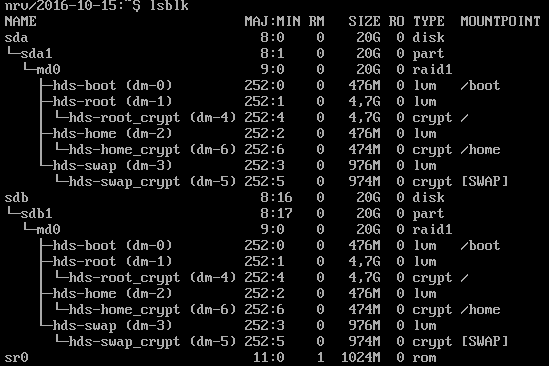
\includegraphics[scale=0.55]{./Imagenes/lsblk-US.png}
		\caption[Comando lsblk ejecutado en Ubuntu Server 14.]{Comando lsblk ejecutado en Ubuntu Server 14.}
	\end{figure}
		
	\section[Cuestión 11.]{Cuestión 11.}
	
	\subsection[a) ¿Cómo ha hecho el disco 2 “arrancable”?]{a) ¿Cómo ha hecho el disco 2 “arrancable”?}
	
	Para que el disco arranque debemos ejecutar el siguiente comando: \cite{grubinstall}
	\begin{lstlisting}[language=bash]
		sudo grub-install /dev/sdb
	\end{lstlisting}
	
	El resultado de la ejecución de dicho comando es:
	
	\begin{figure}[H]
		\centering
		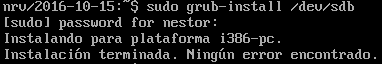
\includegraphics[scale=0.7]{./Imagenes/grub-install.png}
		\caption[Ejecución del comando \textit{sudo grub-install /dev/sdb}.]{Ejecución del comando \textit{sudo grub-install /dev/sdb}}
	\end{figure}
	
	
	\subsection[b) ¿Qué hace el comando grub-install?]{b) ¿Qué hace el comando grub-install?}
	
	Dicho comando instala GRUB en el disco indicado. \cite{grubinstall}
		
	\section[¿Qué diferencia hay entre Standard y Datacenter?]{¿Qué diferencia hay entre Standard y Datacenter?}
	
	Una de las grandes diferencias es el número de instancias que podemos ejecutar a la vez: \cite{instanciasWS2012}
	
	\begin{figure}[H]
		\centering
		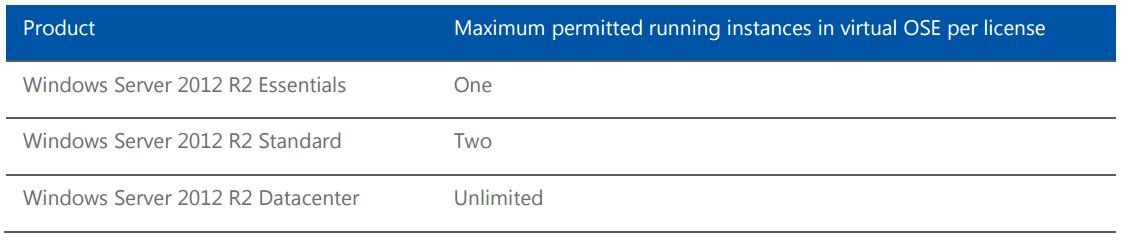
\includegraphics[width=\linewidth]{./Imagenes/instanciasWS2012.png}
		\caption[Número de instancias en Windows Server 2012 R2.]{Número de instancias en Windows Server 2012 R2.}
	\end{figure}
	
	Otra diferencia se trata de una característica llamada \textit{Automatic Virtual Machine Activation}. En el caso de la versión \textit{Standard} sólo está disponible como invitado mientras que en la versión \textit{Datacenter} está disponible como invitado y como host. \cite{standardVSdataventer} \\
	
	Finalmente, otra diferencia es el precio, como podemos observar en la siguiente imagen: \cite{precioWS2012}
	
	\begin{figure}[H]
		\centering
		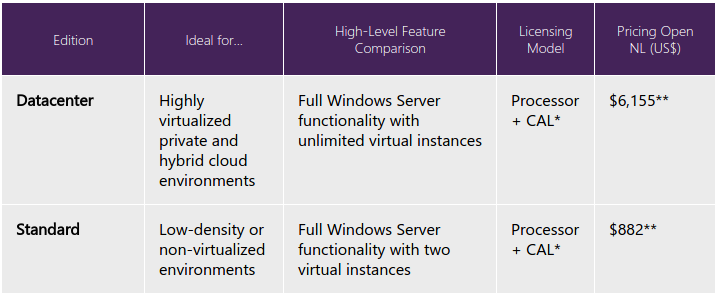
\includegraphics[width=\linewidth]{./Imagenes/precioWS2012.png}
		\caption[Precio Windows Server 2012 R2.]{Precio Windows Server 2012 R2.}
	\end{figure}
	
	
	\section[Continúe usted con el proceso de definición de RAID1 para los dos discos de 50MiB que ha creado. Muestre el proceso con capturas de	pantalla.]{Continúe usted con el proceso de definición de RAID1 para los dos discos de 50MiB que ha creado. Muestre el proceso con capturas de	pantalla.}
	
	\begin{figure}[H]
		\centering
		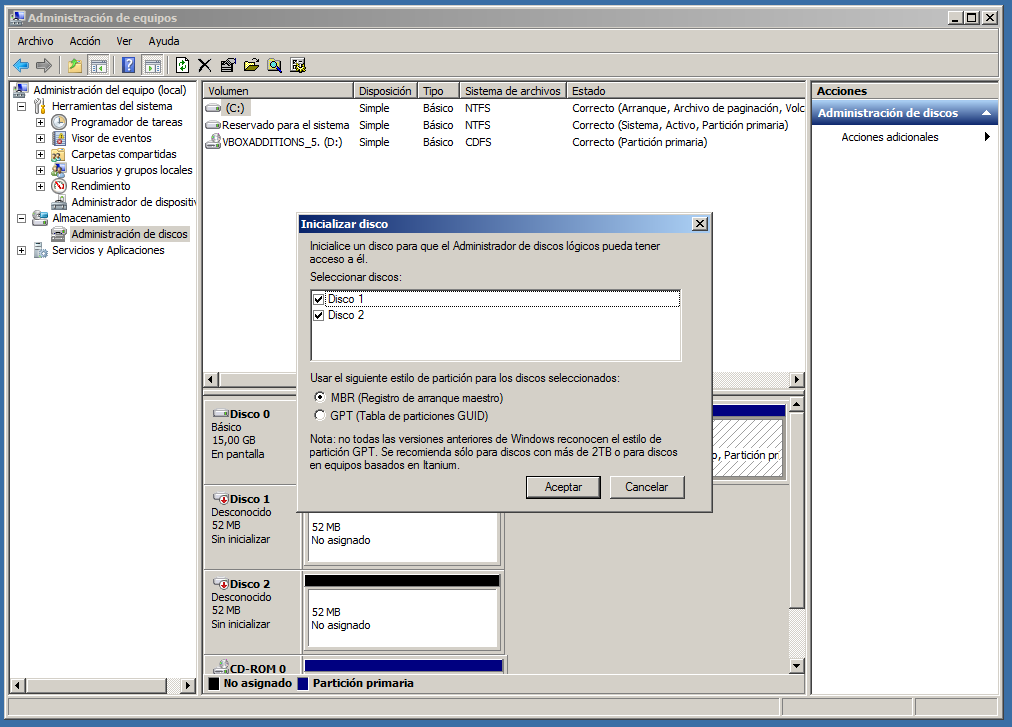
\includegraphics[scale=0.31]{./Imagenes/WSRAIDPaso1.png}
		\caption[Creación de una tabla de particiones.]{Creación de una tabla de particiones.}
		\label{WSRAIDPaso1}
	\end{figure}
	
	\begin{figure}[H]
		\centering
		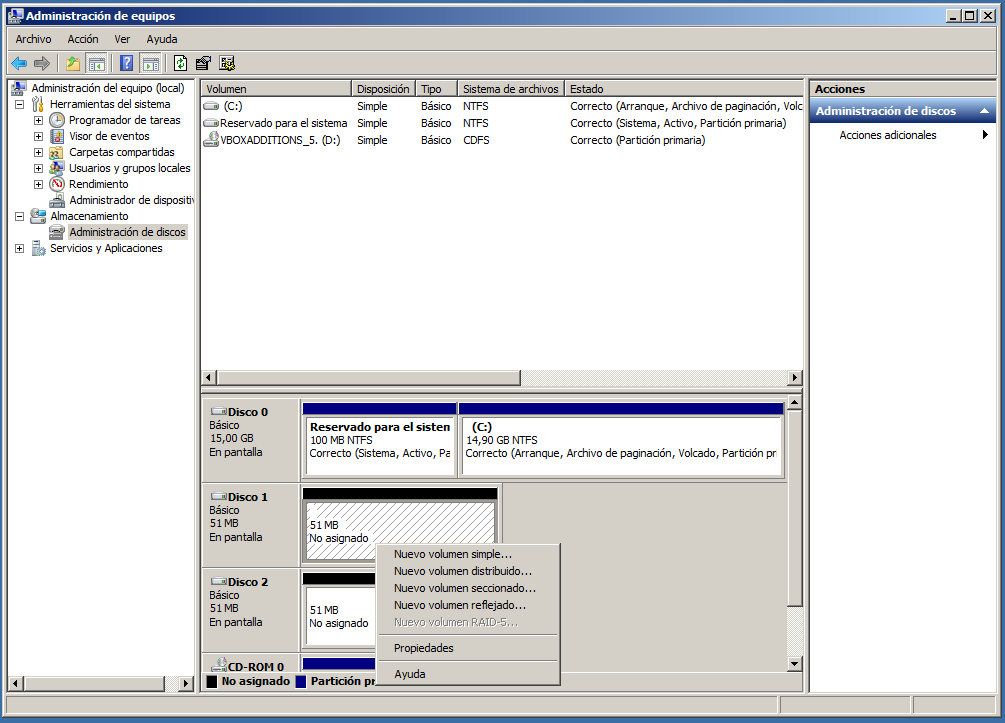
\includegraphics[scale=0.31]{./Imagenes/WSRAIDPaso2.png}
		\caption[Nuevo volumen reflejado.]{Nuevo volumen reflejado.}
		\label{WSRAIDPaso2}
	\end{figure}
		
	\begin{figure}[H]
		\centering
		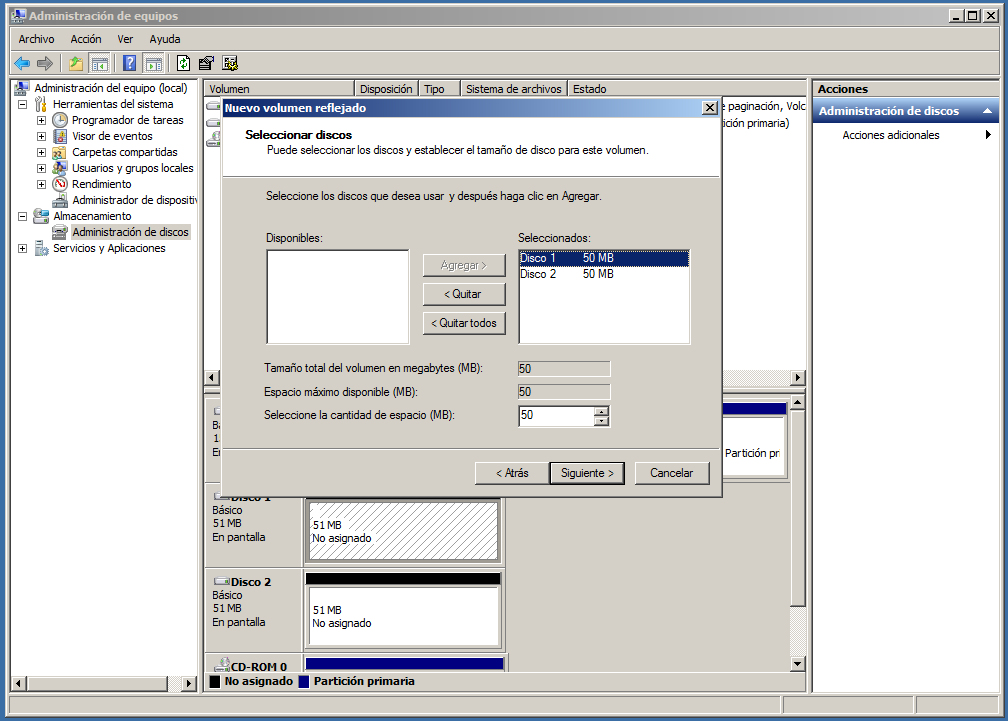
\includegraphics[scale=0.38]{./Imagenes/WSRAIDPaso3.png}
		\caption[Agregación del disco 2.]{Agregación del disco 2.}
		\label{WSRAIDPaso3}
	\end{figure}
	
	\begin{figure}[H]
		\centering
		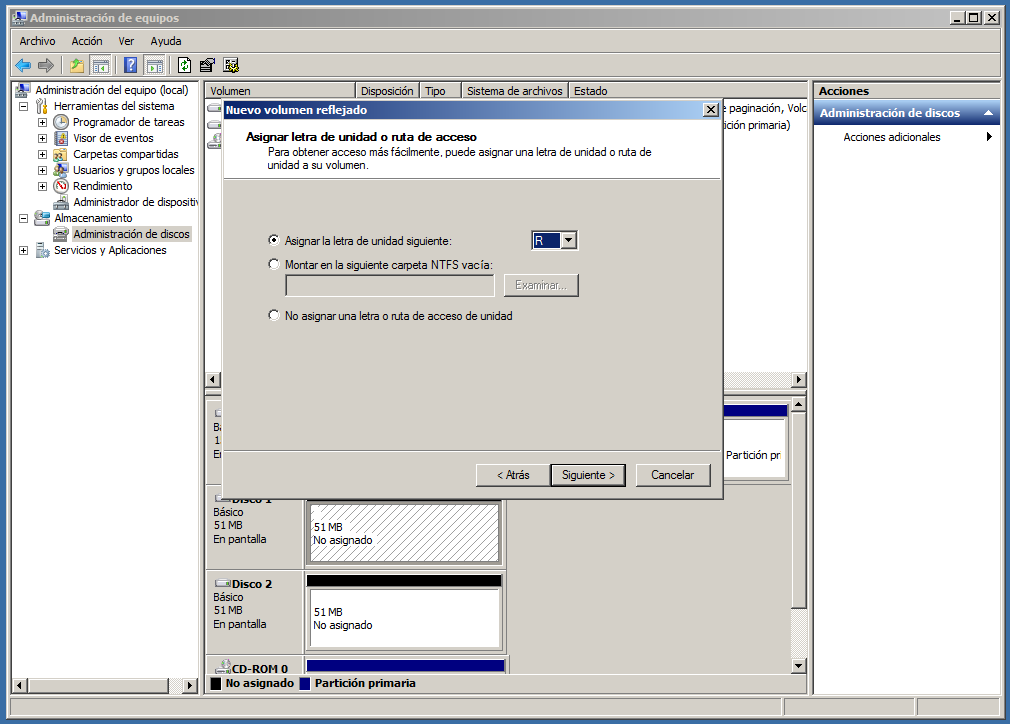
\includegraphics[scale=0.38]{./Imagenes/WSRAIDPaso4.png}
		\caption[Asignación de la letra de unidad al disco.]{Asignación de la letra de unidad al disco.}
		\label{WSRAIDPaso4}
	\end{figure}	
	
	\begin{figure}[H]
		\centering
		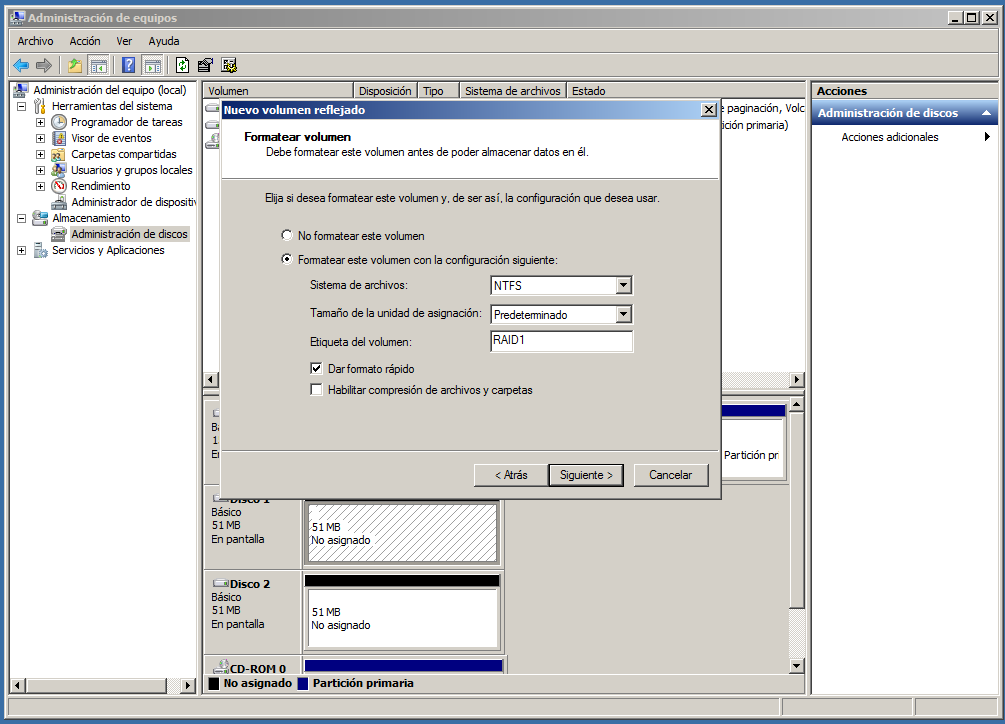
\includegraphics[scale=0.38]{./Imagenes/WSRAIDPaso5.png}
		\caption[Formateo y etiquetado del volumen.]{Formateo y etiquetado del volumen.}
		\label{WSRAIDPaso5}
	\end{figure}
	
	\begin{figure}[H]
		\centering
		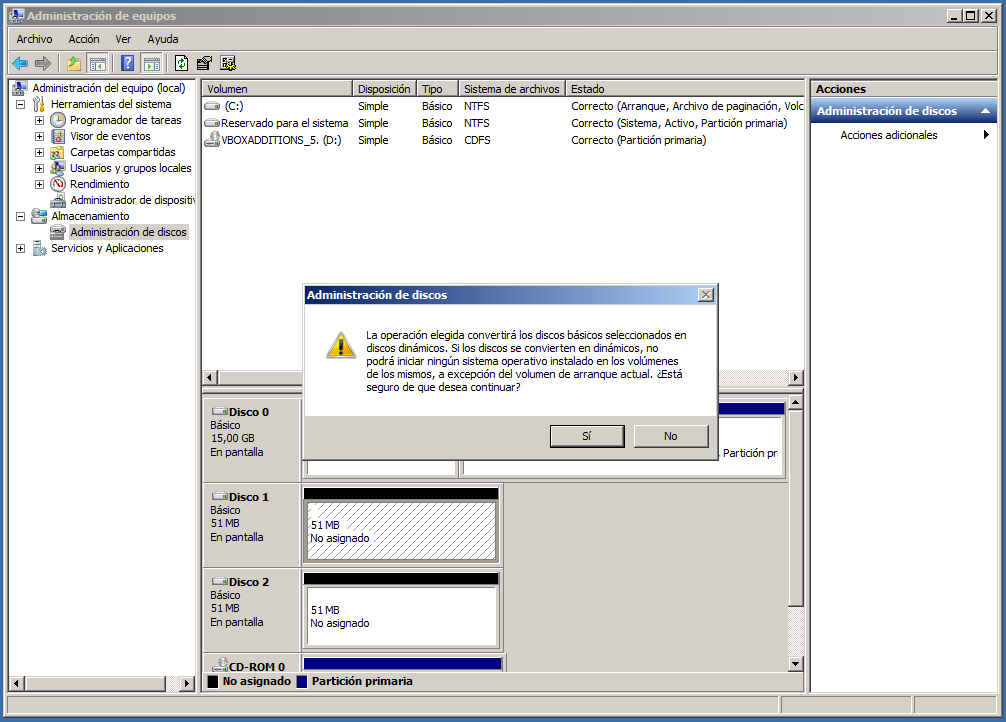
\includegraphics[scale=0.38]{./Imagenes/WSRAIDPaso6.png}
		\caption[Advertencia de que no podrá arrancar un sistema operativo.]{Advertencia de que no podrá arrancar un sistema operativo.}
		\label{WSRAIDPaso6}
	\end{figure}	
	
	\begin{figure}[H]
		\centering
		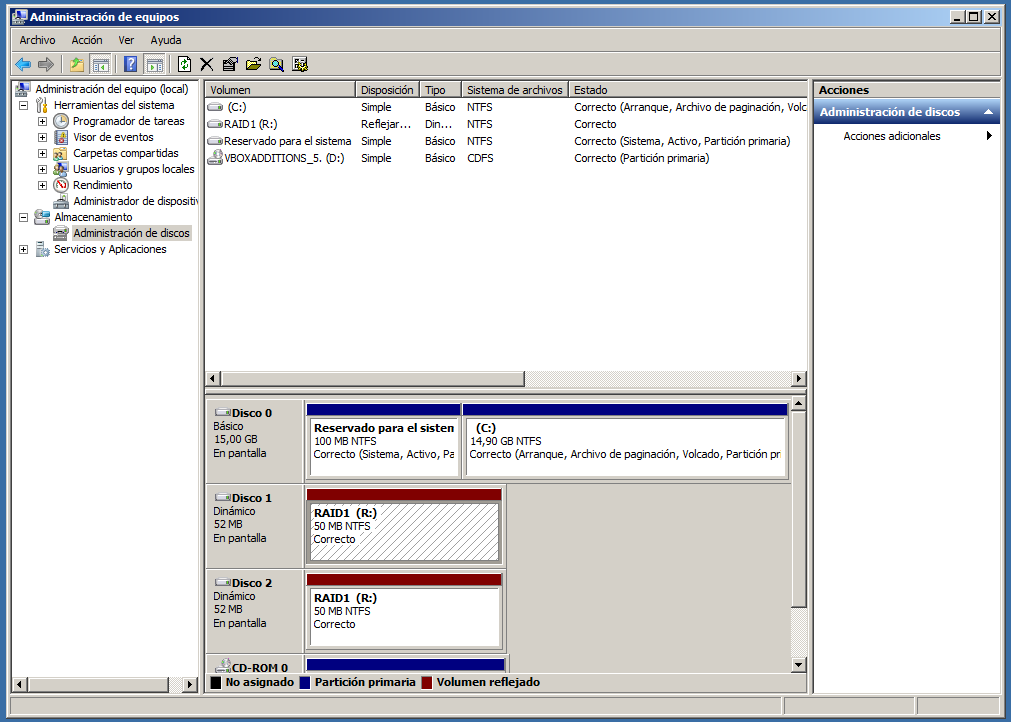
\includegraphics[scale=0.35]{./Imagenes/WSRAIDPaso7.png}
		\caption[RAID configurado.]{RAID configurado.}
		\label{WSRAIDPaso7}
	\end{figure}
	
	Unas cuantas aclaraciones:
	\begin{itemize}
		\item En la figura \ref{WSRAIDPaso2} debemos hacer click derecho sobre el disco de 50 MiB para que aparezca dicho menú.
		\item En la figura \ref{WSRAIDPaso4} he elegido la latra \textit{R} ya que es para el \textit{RAID} y es más fácil de reconocer.
		\item En la figura \ref{WSRAIDPaso5} he etiquetado el volumen como \textit{RAID1} por el mismo motivo que en el punto anterior, para facilitar su reconocimiento posteriormente.
		\item En la figura \ref{WSRAIDPaso6} aceptaremos la advertencia y así finalizará el proceso.
	\end{itemize}
		
	\section[Explique brevemente qué diferencias hay entre los tres tipos de conexión que permite el VMSW para las Mvs: NAT, Host-only y Bridge.]{Explique brevemente qué diferencias hay entre los tres tipos de conexión que permite el VMSW para las Mvs: NAT, Host-only y Bridge.}
	
	Podemos encontrar la respuesta en la página oficial de VirtualBox. \cite{conexionesVMSW}
	
	\begin{itemize}
		\item \textbf{NAT: } (Network Address Translation) es la manera más simple de acceder a una red externa desde una máquina virtual ya que no requiere ninguna configuración especial. Una máquina virtual con NAT activado actúa como un ordenador real que se conecta a Internet a través de un router. El ``router'' en este caso es el motor de red de VirtualBox, el cual mapea el tráfico de red desde y hacia la máquina virtual de manera transparente. En VirtualBox este router esta ubicado entre cada máquina virtual y el host. Esta separación aumenta la seguridad ya que, de este modo, las máquinas virtuales no pueden comunicarse entre ellas.
		\item \textbf{Bridge: } En este modo VirtualBox usa un driver el sistema anfitrión que filtra los datos de tu tarjeta física de red. Este driver se llama \textit{net filter driver}. Esto permite a VirtualBox interceptar el tráfico de la red virtual e introducir datos en el, creando una nueva interfaz de red en el software. Cuando un ``guest'' usa dicha nueva interfaz software, mira al huésped como si estuviese físicamente conectado usando un cable de red: el huésped puede enviar y recibir datos del ``guest'' usando dicha interfaz.				
		\item \textbf{Host-Only: } Este tipo de conexión puede ser visto como un sistema híbrido entre los dos nombrados anteriormente. Como en la conexión de tipo \textit{bridge}, las máquinas virtuales puedes comunicarse entre ellas y el host como si estuviesen físicamente conectadas y como en en la conexión de tipo \textit{NAT} las máquinas virtuales no pueden interactuar con el exterior al host ya que no tiene una conexión física.
	\end{itemize}
	
	\clearpage
	
	\section[Cuestión opcional 1: Muestre (con capturas de pantalla) cómo ha comprobado que el RAID1 funciona.]{Cuestión opcional 1: Muestre (con capturas de pantalla) cómo ha comprobado que el RAID1 funciona.}
	
	Para probar que funciona correctamente vamos a hacer una simulación de fallo y a arreglar el daño causado para ver si el disco se sincroniza correctamente. El proceso es el que sigue: \cite{comprobarRAID} \\
	
	Primero vamos a simular un fallo software. Para ello usamos el comando \textit{sudo mdadm --manage --set-faulty /dev/md0 /dev/sdb1} como se muestra en la figura \ref{comprobacionRAID1}.	
	
	\begin{figure}[H]
		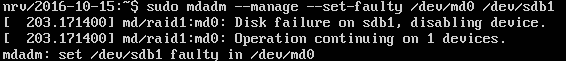
\includegraphics[width=\linewidth]{./Imagenes/ComprobarRAID1.png}
		\vspace{-0.5cm}
		\caption[Simulación fallo software.]{Simulación fallo software.}
		\label{comprobacionRAID1}
	\end{figure}
	
	Para ver que correctamente se ha producido el fallo veremos el estado del disco. Para ello usamos el comando \textit{sudo mdadm --detail /dev/md0} como se muestra en la figura \ref{comprobacionRAID2}.
	
	\begin{figure}[H]
		\centering
		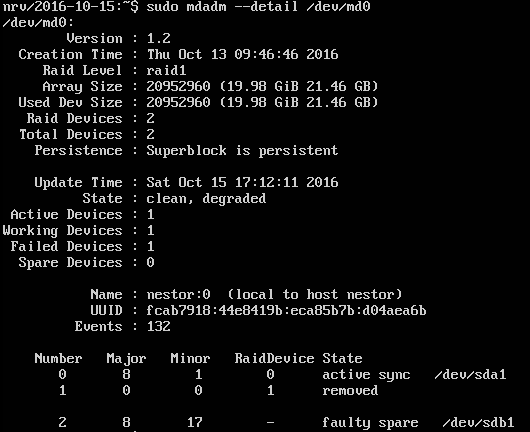
\includegraphics[scale=0.68]{./Imagenes/ComprobarRAID2.png}
		\caption[Comprobación del fallo software.]{Comprobación del fallo software.}
		\label{comprobacionRAID2}
	\end{figure}
	
	Para arreglar el fallo producido vamos a retirar en caliente el disco. Para ello usamos el comando \textit{sudo mdadm /dev/md0 -r /dev/sdb1} como se muestra en la figura \ref{comprobacionRAID3}.	
	
	\begin{figure}[H]
		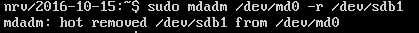
\includegraphics[width=\linewidth]{./Imagenes/ComprobarRAID3.png}
		\vspace{-0.5cm}
		\caption[Retirada en caliente del disco.]{Retirada en caliente del disco.}
		\label{comprobacionRAID3}
	\end{figure}
	
	Para finalizar, volvemos a añadir el disco. Para ello usamos el comando \textit{sudo mdadm /dev/md0 -a /dev/sdb1} como se muestra en la figura \ref{comprobacionRAID4}.
	
	\begin{figure}[H]
		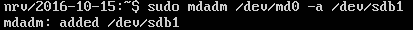
\includegraphics[width=\linewidth]{./Imagenes/ComprobarRAID4.png}
		\vspace{-0.5cm}
		\caption[Añadir el disco a \textit{/dev/sdb1}.]{Añadir el disco a \textit{/dev/sdb1}.}
		\label{comprobacionRAID4}
	\end{figure}
	
	Para ver que todo ha ido correctamente sólo tenemos que comprobar el estado del disco. Para ello usamos el comando \textit{sudo mdadm --detail /dev/md0} como se muestra en la figura \ref{comprobacionRAID5}.
	
	\begin{figure}[H]
		\centering
		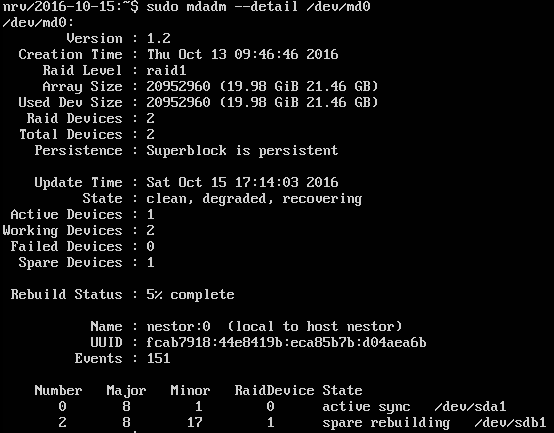
\includegraphics[scale=0.73]{./Imagenes/ComprobarRAID5.png}
		\caption[Comprobación final.]{Comprobación final.}
		\label{comprobacionRAID5}
	\end{figure}
	
	\section[Cuestión opcional 2: ¿Qué relación hay entre los atajos de teclado de emacs y los de la consola bash? ¿y entre los de vi y las páginas del manual?]{Cuestión opcional 2: ¿Qué relación hay entre los atajos de teclado de emacs y los de la consola bash? ¿y entre los de vi y las páginas del manual?}
	
	La relación se debe a que el \textit{bash} se puede poner en varios modos, y uno de ellos es el modo \textit{emacs}. \cite{bashemacs}
	
	La relación es que en ambos se usan los mismos comando. Para ver los comandos que se usan en \textit{man} podemos ejecutar \textit{man man} y a continuación pulsar \textit{h} para ver los diferentes comandos. Los comandos de \textit{vi} podemos verlos en la página de IBM \cite{vi}. Por ejemplo, para ir a la última línea de la página en ambos casos debemos pulsar la tecla \textit{G}.
	
	\clearpage
	\bibliography{bibliografia}
	\bibliographystyle{ieeetr}

\end{document}
